% This is LLNCS.DEM the demonstration file of
% the LaTeX macro package from Springer-Verlag
% for Lecture Notes in Computer Science,
% Version 2.20 of 2017/10/04
%
%\documentclass[runningheads]{llncs}
\documentclass{llncs}
%\usepackage[latin1]

\usepackage[spanish,es-tabla]{babel}
\selectlanguage{spanish}
\usepackage[utf8]{inputenc}
\usepackage{graphicx}
\usepackage{listings}
%
\usepackage{makeidx}
%\usepackage{amsmath}
%\usepackage{mathtools}
\usepackage{hyperref}  % allows for indexgeneration
%
\hyphenation{fun-cio-na-li-dad}
\begin{document}
%

%
%\title{BUE: El algoritmo que eligió al Gobernador}
%\title{Informe Fiscalización Informática}
\title{Comparación BUP - BUE - Boletas Partidarias}
\subtitle{Ventajas de la Boleta Única en Papel}
%

%\title{Hamiltonian Mechanics2}


\author{ Pablo Kogan, Silvia Soto, Claudio Vaucheret }


\institute{
%Grupo de Investigación en Lenguajes e Inteligencia Artificial\\Departamento de Teoría de la Computación - 
Facultad de Informática\\
Universidad Nacional del Comahue \\
\email{\{pablo.kogan,silvia.soto,cv\}@fi.uncoma.edu.ar}
}
\maketitle              % typeset the title of the contribution
%
\begin{abstract}
En los últimos años se han planteado cambios a los procesos del sistema electoral a nivel universitario, municipal, provincial y nacional hacia enfoques variados. 
En algunos municipios y provincias Argentinas ya se utilizan sistemas de voto electrónico, cambiando las formas y reglas de administración electoral sobre las diferentes fases de la elección.
%En la provincia de Neuquén se utilizó por primera vez el sistema de Boleta Única Electrónica, y 
La experiencia de las siete elecciones realizadas utilizando el sistema Gukena en las Elecciones de la Universidad Nacional del Comahue, ha impactado de manera positiva en la construcción de confianza en el proceso de electoral, principalmente porque los datos del acta son ingresados al sistema por el responsable del mismo, la autoridad de mesa, y además por la mejora en la velocidad en la obtención y publicación de los resultados.  

La combinación de Gukena con boleta única en papel y conteo manual, ofrece todas las ventajas que proponen los sistemas de voto electrónico y además constituye un solución menos costosa que elimina posibles vulnerabilidades en cuanto al secreto e integridad del voto.
Por esta razón, se propone modificar base normativa de la Universidad para afianzar el proceso utilizado y cambiar de múltiples boletas papel a boleta única papel.

En este trabajo describimos las ventajas de la utilización de Boleta Única en Papel en las elecciones de la Universidad Nacional del Comahue, en contraste con los sistemas de Boletas Partidarias y Boleta Única Electrónica.

%trata de la investigación y el desarrollo de una innovación tecnológica a nivel informático para mejorar el proceso de computo de las elecciones de la Universidad Nacional del Comahue.

\keywords{Voto Electrónico. Desarrollo de software. Fundamentación BUP. BUE}
\end{abstract}
%

\section{Introducción}
%

El sistema de votación utilizado en Argentina debe proteger los derechos del elector al asegurar universalidad, igualdad, obligatoriedad y confidencialidad del voto. La transparencia del sistema electoral genera la confianza de todos los participantes: Electores, Autoridades de Mesa, Partidos Políticos, la Justicia Electoral y el Estado sobre la legitimidad de los resultados y de todo el proceso.
% cambié votantes por electores y Agrupaciones políticas por Partidos Políticos (así los nombre el código electoral

%Una elección
Si bien el momento de votación y el escrutinio son las etapas que cobran más visibilidad, en \cite{conicet} se plantea un modelo de referencia que identifica 5 fases entre el acto electoral y escrutinio provisorio:
\begin{itemize}
%\item apertura de mesa
%\item Identificación del Votante
\item Emisión del Voto
\item Escrutinio de la Mesa
\item Generación de Documentos
\item Comunicación de resultados
\item Procesamiento de Resultados y Publicación
\end{itemize}

\begin{figure}
\begin{center}
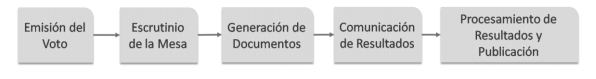
\includegraphics[width=12cm]{img/fases.png}
\end{center}
\caption{Fases del Proceso de Votación}
\label{1fig}
\end{figure}

Cada una de estas etapas deben ser tomadas con igual importancia al momento de su fiscalización, ya que un error en cualquiera de ellas puede afectar todo el proceso electoral.

Se puede agregar tecnología automatizando cualquiera de estas fases, pero se considera 'Voto Electrónico' a cualquier sistema que introduzca computadoras en la Emisión del Voto y/o el Escrutinio de la Mesa.  
%identificar puntos problemáticos

Se han identificado numerosas vulnerabilidades en cuanto al  secreto e integridad del voto en las experiencias de Voto Electrónico realizadas en el país y en el exterior.  Se han identificado altos riesgos en las fases de Emisión del Voto y Escrutinio de la Mesa en el país \cite{amato2015vot,chaparro2016sistema,nardi2017voto} y el exterior \cite{jacobs2009electronic,aranha2014software,suiza}. Sin embargo en el ámbito local se ha avanzado en lo normativo, creando Leyes y Ordenanzas \cite{leyprovincia}\cite{ordenanzamuni}, para implementar el sistema de Boleta Única Electrónica a nivel Provincial y Municipal.  

%ver contexto nacional acerca de los cambios en el proceso

A nivel Nacional, en contraste y a pesar de varios intentos de incluir el voto electrónico, solo se han introducido cambios más cautos, por iniciativa del Poder Judicial de la Nación  \cite{poderJudicial}, con respecto a agregar tecnología solamente a la fase de comunicación de resultados. En las elecciones presidenciales de 2019 se permitió para el escrutinio provisorio que las actas de escrutinio sean digitalizados y transmitidos desde el propio establecimiento de votación y por las propias autoridades de mesa, manteniendo la boleta papel y el conteo manual, y se lograron buenos resultados en cuanto velocidad de computo.

%La transición entre un sistema con boleta papel a un sistema de voto electrónico provoca cambios en las formas tradicionales de fiscalización a la que las agrupaciones políticas y las justicias electorales están acostumbradas.  Los fiscales informáticos y fiscales de mesa deben modificar sus tareas para controlar que el sistema funcione de manera correcta.  

En la Universidad Nacional del Comahue se realizan elecciones, todos los años y para los diferentes claustros, utilizando el método tradicional de boleta papel, conteo manual y elaboración del acta de escrutinio manual. Desde el año 2015  se usa el sistema Gukena \cite{soto2018gukena} para mejorar la Comunicación de los Resultados y el Escrutinio provisorio con muy buenos registros en cuanto a la velocidad en que se obtienen los resultados.   El mismo, permite a las autoridades de mesa ingresar los datos al sistema de escrutinio directamente desde el lugar de votación  \cite{rionegro}. 


%Identificar procesos. Proceso de votación - proceso de recuentos

%2) Definir voto electrónico - identificar puntos problemáticos. \cite{sadio}
%misión crítica \cite{conicet}

%3) identificar en el recuento de votos como un sub sistema susceptible a ser intervenido sin  dañar las fortalezas nombradas en 1)

%4) decribir la propuesta Base normartiva + sistema 





%El sistema se encuentra disponible en el sitio web de la universidad desde Mayo de 2015. 

%Experiencias en otros lugares del país y del exterior.

%\section{Problema de Investigación}
%Gukena es un Sistema Web que permite el escrutinio descentralizado de elecciones, desarrollado por estudiantes de la Facultad de Informática de la Universidad Nacional del Comahue.


\section{Boleta Única Papel}
%Describir la importancia de lo que se decide con la elección
Que es la Boleta Única Papel 

\subsection{Experiencias}

\subsection{Ventajas}
Robo de Boletas
Transparencia
Ahorro de Papel
Fiscalización
Mini-Cuarto Oscuro

\subsection{Modelo de BUP}

\subsection{Proceso Emisión Voto}

\subsection{Proceso de Conteo}

\section {BUE}
Experiencia del año pasado
- Situación Gobernador
- Encuesta
- Caso Centenario

\section{Comparación}
Comparación por BUE - BUP - BP

\begin{itemize}
\item Apertura de mesa
%\item Identificación del Votante
\item Emisión del Voto
\item Escrutinio de la Mesa
\item Generación de Documentos
\item Comunicación de resultados
\item Procesamiento de Resultados y Publicación
\end{itemize}










\section{Conclusiones y Propuestas de Mejora}




%\section{Agradecimientos}

%Las actividades concretadas en el ámbito de esta investigación se plantean articuladas a la Extensión Universitaria buscando promover que estudiantes avanzados de la Facultad de Informática trabajen en un desarrollo real para la Universidad del Comahue con intención de construir y ampliar conocimiento a partir de la revisión y análisis de resultados desarrollados en el campo de la praxis.



%Entrevistas a Chacareros que utilizaron el semáforo ???
%Enlo que respecta a los materiales y métodos no se especifica una metodología de validación del desarrollo realizado, ni ensayos, solo una descripción del desarrollo realizado. Me parece un buen trabajo a nivel de comunicación de avances de un desarrollo, pero considero le falta alguna metodología de verificación y ensayos, para ser considerado un trabajo científico.

%Respecto a la validación de los resultados, no me imagino como se puede hacer, ya que los datos son los que ocurren por las condiciones climáticas y no hay mucho más para hacer. Lo único que se podría hacer es respetar las condiciones de aplicación para el control de alguna plaga durante una temporada en alguna chacra y en otra, no (con sus respectivas repeticiones) y luego comparar los resultados del control de esa plaga, pero sería como probar que el sol todos los días sale por el este….De todas maneras eso sería para el año que viene.
%Otra forma de evaluarlo podría ser analizando el número de entradas a la página para ver la aplicación….no sé, no se me ocurre mucho más.

%
% ---- Bibliography ----
\bibliographystyle{plain}
\bibliography{refer}
\end{document}
